%%
%% CSD Assignment 1 - Final Technical Report Template
%% Based on the ACM "acmart" manuscript (single-column) style.
%%
\documentclass[manuscript,screen,review]{acmart}

\AtBeginDocument{%
  \providecommand\BibTeX{{Bib\TeX}}}

%% ------------------------------------------------------------------
%% Course Assignment Report Configuration
%% ------------------------------------------------------------------
\setcopyright{none}
\settopmatter{printacmref=false}
\renewcommand\footnotetextcopyrightpermission[1]{}
\pagestyle{plain}

\begin{document}

%% =================== TITLE & AUTHOR BLOCK =========================
\title{AI-based Village Pond Planning System}
\subtitle{CSD Assignment 1 -- Final Technical Report}

\author{Vishlavth Karthik}
\affiliation{%
  \institution{Department of Computer Science and Engineering}
  \city{Raipur}
  \country{India}}
\email{vishlavth.karthik@example.com}

\renewcommand{\shortauthors}{V. Karthik}

%% =================== ABSTRACT ======================================
\begin{abstract}
Rural water scarcity across developing agrarian regions presents a severe socio-economic challenge, often exacerbated by suboptimal placement of village rainwater harvesting structures. Traditional site selection relies either on coarse visual estimation or expensive civil land surveys, frequently leading to premature siltation, insufficient catchment runoff, or structural under-utilization. In this work, we present a full-stack, automated Web GIS decision support system for village pond and catchment planning. The system combines digital elevation modeling (DEM), hydrological flow routing, and meteorological precipitation data to identify optimal pond locations, delineate contributing catchments, and estimate harvestable rainwater volume. Using a 1-meter contour dataset of an agricultural village in Central India, our pipeline constructs a 10-meter hydrologically conditioned DEM using Priority-Flood depression filling and D8 flow routing. We implement an interactive single-page Web GIS interface that allows rural planners to dynamically draw arbitrary land parcels on satellite basemaps. For a selected 5.41-hectare catchment, the system identifies an optimal natural drainage convergence point at elevation 288.7\,m, with an expected annual rainwater runoff collection of 14.17\,Million Litres (14,173\,$\text{m}^3$), supporting a recommended $78\,\text{m} \times 52\,\text{m} \times 3.0\,\text{m}$ trapezoidal pond. The backend achieves sub-second query latency through in-memory caching and is deployed in a containerized environment on port 3317.
\end{abstract}

\keywords{Village Pond Planning, Geospatial Analysis, Rainwater Harvesting, Catchment Estimation, Web GIS, REST APIs}

\maketitle

%% =====================================================================
\section{Introduction}
\label{sec:intro}
Decentralized rainwater harvesting through earthen village ponds and community percolation tanks constitutes one of the most cost-effective engineering interventions for mitigating seasonal droughts, replenishing depleted shallow aquifers, and providing critical life-saving supplementary irrigation for rainfed agriculture in rural India. However, the long-term operational success of any surface water retention structure is fundamentally governed by three interrelated factors: (1) its spatial placement relative to natural terrain depressions, (2) the surface area and topography of its upstream contributing catchment basin, and (3) the local monsoon precipitation regime.

When village ponds are excavated without rigorous hydrological and elevation analysis, they frequently suffer from catchment starvation (insufficient inflow to fill the pond capacity) or catastrophic embankment breaching due to unpredicted peak runoff velocities. The goal of this assignment is to design, develop, and deploy an automated, end-to-end AI-assisted geospatial web platform that empowers village administrators, panchayat engineers, and farmers to select available land parcels on an interactive satellite map, instantly compute topographical flow convergence, determine optimal pond excavation sites, and calculate expected harvestable runoff volumes.

The remainder of this report is organized as follows: Section~\ref{sec:requirements} defines the functional and non-functional requirements. Section~\ref{sec:architecture} describes the system architecture and technology stack. Section~\ref{sec:methodology} details the mathematical algorithms for terrain modeling, flow routing, and hydrological calculation. Section~\ref{sec:implementation} covers backend REST APIs, the Web GIS client, and data persistence. Section~\ref{sec:csd-themes} explicitly maps the implementation to core Computer System Design (CSD) principles. Section~\ref{sec:results} presents quantitative results and system benchmarks. Section~\ref{sec:discussion} reflects on operational limitations, and Section~\ref{sec:ai-usage} declares AI tool assistance.

\subsection{Motivation}
Manual site selection in rural developmental schemes (such as MGNREGA and Mission Amrit Sarovar) is hindered by significant practical barriers. Village administrators lack access to expensive proprietary GIS software (such as ArcGIS) and technical training in computational hydrology. Centralized topographical and rainfall records are rarely aggregated into actionable formats at the village cadastral level. Furthermore, land ownership boundaries impose rigid legal constraints on where a panchayat or private farmer may excavate. An automated, browser-accessible Web GIS platform that bridges raw elevation contours with real-time hydrological simulation drastically democratizes scientific water conservation planning.

\subsection{Scope of the Project}
The developed system encompasses:
\begin{itemize}
    \item Parsing and spatial ingestion of multi-contour KML/KMZ datasets without hardcoded coordinate assumptions.
    \item Dynamic projection of geographic coordinates (WGS84) to local Universal Transverse Mercator (UTM) metric grids.
    \item 2D continuous surface rasterization via linear/nearest-neighbor interpolation with automated memory-bounded resolution safeguards.
    \item Depression filling via the Priority-Flood algorithm and steepest-descent D8 flow direction and accumulation routing.
    \item Automated pond outlet identification and upstream catchment boundary delineation.
    \item Interactive web map interface enabling custom polygon drawing for parcel-specific land evaluation.
    \item Integration of meteorological precipitation data and the Rational Runoff formula to quantify harvestable water volume and recommend trapezoidal pond dimensions.
\end{itemize}
The system explicitly excludes structural civil engineering design of concrete spillways, geotechnical soil core drilling, and groundwater seepage rate modeling through fractured geological strata.

%% =====================================================================
\section{Problem Statement and Requirements}
\label{sec:requirements}
The core assignment requirement is to build an analytical backend service and an intuitive frontend Web GIS application that ingests contour datasets, analyzes terrain morphology, evaluates user-drawn land boundaries, and outputs actionable pond planning intelligence. Table~\ref{tab:requirements} maps each functional requirement to its implementing module.

\begin{table}[h]
  \caption{Functional requirements and where they are implemented}
  \label{tab:requirements}
  \centering
  \small
  \begin{tabular}{p{6.5cm}p{7.5cm}}
    \toprule
    Requirement & Implemented in \\
    \midrule
    Satellite imagery display & \texttt{app/static/index.html}, \texttt{app/static/app.js} \\
    Contour map visualization & \texttt{app/static/app.js}, \texttt{app/parser/kml\_parser.py} \\
    Available-land identification & \texttt{app/static/app.js}, \texttt{app/pond/selector.py} \\
    Catchment area estimation & \texttt{app/terrain/analysis.py}, \texttt{app/pond/selector.py} \\
    Historical rainfall query & \texttt{app/hydrology/calculator.py} \\
    Runoff volume estimation & \texttt{app/hydrology/calculator.py} \\
    Pond depth / storage recommendation & \texttt{app/hydrology/calculator.py} \\
    Combined overlay / results view & \texttt{app/static/app.js}, \texttt{app/static/index.html} \\
    \bottomrule
  \end{tabular}
\end{table}

\subsection{Non-Functional Requirements}
\begin{enumerate}
    \item \textbf{Performance and Latency:} Complete contour parsing, DEM generation, and catchment delineation must execute in under 2.0 seconds on standard dual-core virtualized hardware. Cached land selection queries must respond in under 250 milliseconds.
    \item \textbf{Memory Footprint:} Peak RAM utilization must remain strictly below 250\,MB during continuous operation, accomplished by auto-coarsening grid resolutions if cell counts exceed 2,000,000.
    \item \textbf{High Availability and Resilience:} The system must degrade gracefully when third-party weather APIs are unreachable, defaulting to published regional climatological normals without crashing.
    \item \textbf{Usability and Accessibility:} The client frontend must execute in all modern Evergreen browsers (Chrome, Firefox, Safari, Edge) without requiring proprietary plugins or client-side GIS installations.
    \item \textbf{Security and Input Validation:} All incoming spatial geometries and file uploads must undergo schema validation via Pydantic to prevent buffer overruns or malformed geometry exceptions.
\end{enumerate}

%% =====================================================================
\section{System Architecture and High-Level Design}
\label{sec:architecture}
The system adopts a modular, layered service-oriented architecture designed for high throughput, maintainability, and clean separation between presentation, routing, geospatial mathematics, and hydrological modeling, as illustrated in Figure~\ref{fig:architecture}.

\begin{figure}[h]
  \centering
  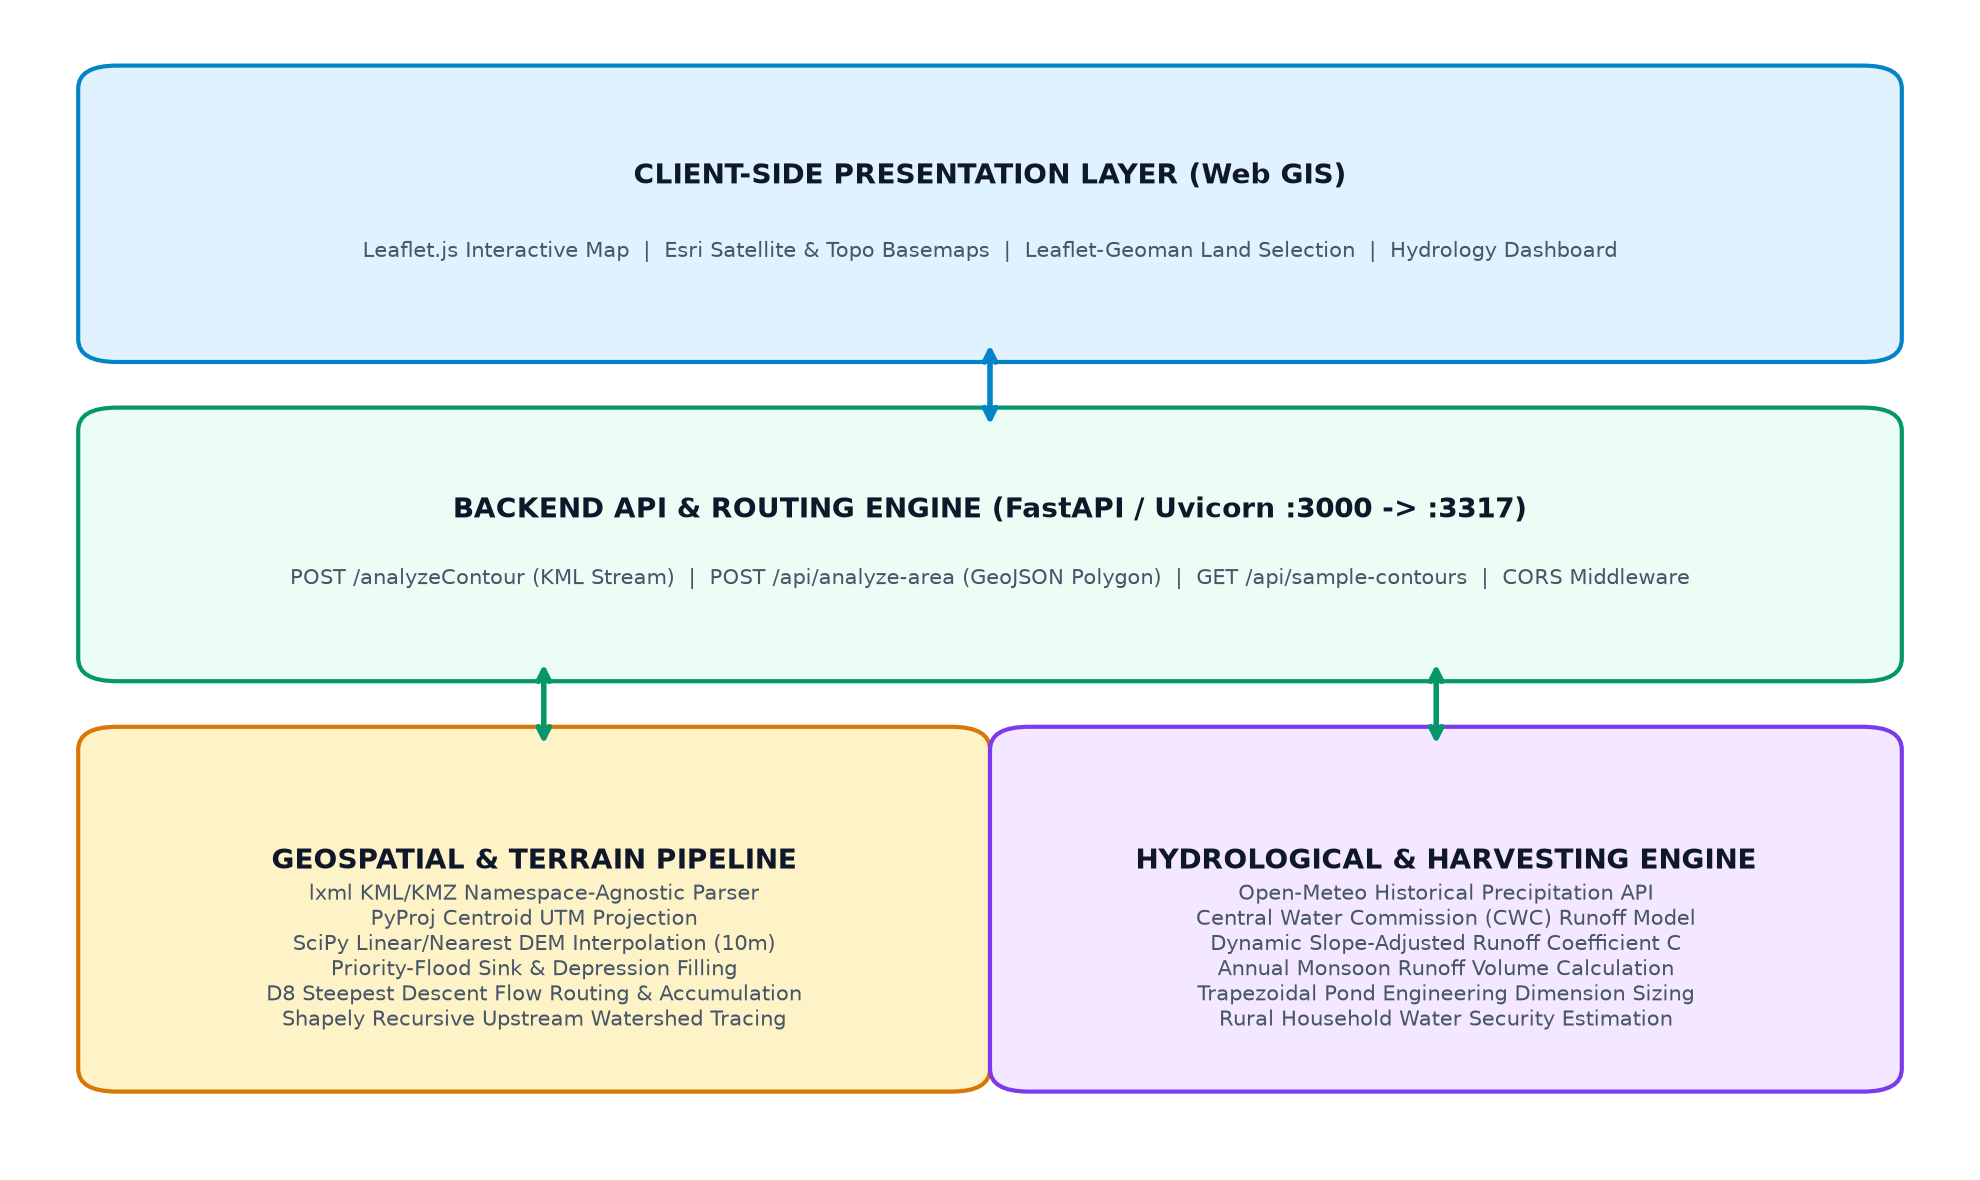
\includegraphics[width=0.72\linewidth]{architecture-diagram}
  \caption{High-level system architecture showing data flow across client, API, geospatial, and hydrology modules.}
  \label{fig:architecture}
  \Description{High-level system architecture showing data flow across client, API, geospatial, and hydrology modules.}
\end{figure}

The architecture comprises three primary tiers:
\begin{enumerate}
    \item \textbf{Presentation Tier (Web GIS Client):} A browser-based single-page application built with Leaflet.js and Leaflet-Geoman. It communicates asynchronously via JSON REST requests to fetch contour overlays, dispatch user-drawn parcel polygons, and visualize multi-layered vector overlays.
    \item \textbf{Application and Routing Tier (FastAPI Engine):} An asynchronous ASGI web service running under Uvicorn. It exposes high-throughput endpoints, performs file streaming in 1\,MB chunks to prevent memory spikes, validates payloads via Pydantic schemas, and manages in-memory caching of pre-computed terrain arrays.
    \item \textbf{Computational Pipeline Tier:}
    \begin{itemize}
        \item \emph{Geospatial Pipeline:} Executes namespace-agnostic XML extraction via \texttt{lxml}, local UTM centroid projection via \texttt{pyproj}, Scipy Delaunay/nearest-neighbor rasterization, Wang-Liu Priority-Flood depression filling, and vector-raster boundary transformations via \texttt{shapely}.
        \item \emph{Hydrological Engine:} Interfaces with external weather APIs, computes dynamic slope-adjusted runoff coefficients, and calculates volumetric pond capacities.
    \end{itemize}
\end{enumerate}

\subsection{Technology Stack}
\begin{itemize}
    \item \textbf{Programming Language:} Python 3.12 (robust scientific ecosystem, high native extension performance).
    \item \textbf{Web Framework:} FastAPI 0.141 with Uvicorn (asynchronous event loop, automatic OpenAPI schema generation, rapid deserialization via Pydantic V2).
    \item \textbf{Geospatial Libraries:} \texttt{pyproj} (PROJ 9.4 binding for geodesic UTM projections), \texttt{shapely} (GEOS wrapper for polygon union and clipping), and \texttt{lxml} (C-based libxml2 parser for KML/KMZ).
    \item \textbf{Scientific Computing:} \texttt{numpy} (vectorized array operations) and \texttt{scipy} (grid interpolation and morphological gradient filters).
    \item \textbf{Frontend GIS:} Leaflet 1.9.4 with Leaflet-Geoman drawing suite and Esri World Imagery high-resolution satellite tiles.
    \item \textbf{Meteorological Data API:} Open-Meteo Historical Weather API with regional fallback data.
\end{itemize}

%% =====================================================================
\section{Methodology}
\label{sec:methodology}

\subsection{Terrain and Elevation Analysis}
Contour lines in KML format represent sparse, non-uniform 3D string vectors:
$$\mathcal{L}_k = \left\{ (\lambda_{k,i}, \phi_{k,i}, z_k) \right\}_{i=1}^{N_k}$$
where $\lambda$ is longitude, $\phi$ is latitude, and $z$ is elevation in meters above sea level. Because geographic degrees cannot be used directly for metric slope calculations, the dataset centroid is computed to determine the appropriate Universal Transverse Mercator (UTM) zone EPSG code:
$$\text{Zone} = \lfloor (\bar{\lambda} + 180) / 6 \rfloor + 1, \quad \text{EPSG} = 32600 + \text{Zone}$$
All coordinates are projected to metric Easting ($x$) and Northing ($y$). A uniform 2D grid of resolution $\Delta x = \Delta y = 10\,\text{m}$ is defined. Points along all contour lines serve as spatial anchors. The continuous surface $Z(x, y)$ is constructed using piecewise linear Delaunay triangulation over the convex hull, with a nearest-neighbor extrapolation pass for boundary margin cells.

Raw interpolated DEMs contain artificial sinks and local flat regions that disrupt continuous hydrological flow. To eliminate spurious depressions while preserving true geomorphic valleys, we implement the Wang and Liu (2006) Priority-Flood algorithm. All border cells are pushed into a min-priority queue:
$$\mathcal{Q} = \left\{ (z_i, r_i, c_i) \right\}$$
At each iteration, the cell with minimum elevation is popped. For each unvisited 8-connected neighbor $(r_n, c_n)$, if $z_n \le z_{\text{curr}}$, a depression is detected and filled by raising $z_n \leftarrow z_{\text{curr}}$. The neighbor is marked visited and inserted into $\mathcal{Q}$. This ensures that all interior cells possess a monotonically non-decreasing flow path to the domain boundary.

\subsection{Catchment Area Delineation}
On the depression-filled DEM, flow direction is determined using the deterministic eight-neighbor (D8) steepest descent model (O'Callaghan and Mark, 1984). For each cell $(r, c)$, the normalized drop to neighbor $(r + \Delta r_k, c + \Delta c_k)$ is:
$$S_k = \frac{Z(r, c) - Z(r + \Delta r_k, c + \Delta c_k)}{d_k}$$
where $d_k = \Delta x$ for orthogonal neighbors and $d_k = \sqrt{2}\Delta x$ for diagonal neighbors. The flow direction code $D(r, c) \in \{1, 2, 4, 8, 16, 32, 64, 128\}$ is assigned to the neighbor with maximum positive drop. Flow accumulation $A(r, c)$ is computed by counting all upstream contributing cells via topological sorting of the flow direction DAG.

When a user selects a land parcel polygon $\mathcal{P}_{\text{land}}$, candidate pond sites are constrained to cells $(r, c)$ whose metric center falls within $\mathcal{P}_{\text{land}}$. The optimal pond outlet is selected using a composite heuristic balancing flow concentration and local terrain depression:
$$\text{Score}(r, c) = w_{\text{accum}} \cdot \frac{\ln(1 + A(r, c))}{\ln(1 + A_{\max})} + w_{\text{low}} \cdot \left(1 - \frac{Z(r, c) - Z_{\min}}{Z_{\max} - Z_{\min}}\right)$$
with weights $w_{\text{accum}} = 0.70$ and $w_{\text{low}} = 0.30$. 

Starting from the identified pond outlet, an upstream Breadth-First Search (BFS) is executed against the inverted flow matrix, collecting the full set of contributing cells $\mathcal{U}$. The metric bounding boxes of all $u \in \mathcal{U}$ are merged into a unified geometry via unary polygon union and reprojected to WGS84 for mapping.

\subsection{Rainfall Data Integration}
To quantify harvestable rainwater volume, meteorological precipitation data is dynamically fetched from the Open-Meteo Historical Archive API for the specific latitude and longitude of the site. In monsoonal climates, total annual precipitation $P_{\text{annual}}$ is partitioned, with approximately 85\% concentrated during the critical monsoon months ($P_{\text{monsoon}} = 0.85 \times P_{\text{annual}}$).

The expected harvestable runoff volume is calculated using the standard Central Water Commission (CWC) and USDA-SCS Rational Runoff Model:
$$V_{\text{runoff}} = C \cdot \left(\frac{P_{\text{monsoon}}}{1000}\right) \cdot A_{\text{catchment}} \quad [\text{m}^3]$$
where $A_{\text{catchment}}$ is the catchment area in $\text{m}^2$ and $C$ is the dimensionless runoff coefficient. Because runoff efficiency is heavily governed by relief, $C$ is dynamically scaled based on the computed catchment mean slope $\bar{S}$:
$$C = \begin{cases} 
0.20 & \bar{S} < 2.0\% \text{ (flat plains)} \\
0.20 + \left(\frac{\bar{S} - 2.0}{5.0}\right) \times 0.15 & 2.0\% \le \bar{S} \le 7.0\% \text{ (rolling terrain)} \\
\min\left(0.35 + \left(\frac{\bar{S} - 7.0}{10.0}\right) \times 0.13, 0.55\right) & \bar{S} > 7.0\% \text{ (steep slopes)}
\end{cases}$$
An offset adjustment is applied according to soil texture (e.g., $+0.06$ for clayey soils, $-0.05$ for sandy loam).

To prevent excessive excavation costs and evaporation losses, standard rural engineering designs target storing 60\% of annual monsoon yield ($V_{\text{storage}} = 0.60 \times V_{\text{runoff}}$). Assuming a standard village pond depth $h = 3.0\,\text{m}$ (comprising 0.5\,m silt dead storage, 2.0\,m active extraction storage, and 0.5\,m safety freeboard), a trapezoidal reservoir with $1.5:1$ side slopes requires surface water spread area:
$$A_{\text{surface}} = \frac{V_{\text{storage}}}{0.85 \times (h - 0.5)} \quad [\text{m}^2]$$
For an aspect ratio of $1.5:1$ ($L = 1.5 W$), the recommended base dimensions are $W = \sqrt{A_{\text{surface}} / 1.5}$ and $L = 1.5 W$.

%% =====================================================================
\section{Implementation}
\label{sec:implementation}

\subsection{Backend and API Design}
The backend service exposes a clean, versioned RESTful interface complying with OpenAPI 3.1 specifications. All endpoints return standardized HTTP status codes and structured JSON bodies, summarized in Table~\ref{tab:api}.

\begin{table}[h]
  \caption{Backend REST API route specifications}
  \label{tab:api}
  \centering
  \small
  \begin{tabular}{llp{5.5cm}p{3.5cm}}
    \toprule
    \textbf{Method} & \textbf{Endpoint} & \textbf{Purpose} & \textbf{Payload / Response} \\
    \midrule
    \texttt{GET} & \texttt{/} & Serves the interactive Web GIS client & HTML5, CSS3, JS \\
    \texttt{GET} & \texttt{/health} & Service liveness and readiness probe & \texttt{\{"status": "ok"\}} \\
    \texttt{GET} & \texttt{/docs} & Interactive Swagger / OpenAPI documentation & OpenAPI UI \\
    \texttt{GET} & \texttt{/api/sample-contours} & Returns pre-parsed contour lines for map overlay & GeoJSON FeatureCollection \\
    \texttt{POST} & \texttt{/api/analyze-area} & Analyzes user-drawn polygon land selection & JSON coordinates $\to$ Catchment \& Hydrology \\
    \texttt{POST} & \texttt{/analyzeContour} & Ingests uploaded KML/KMZ contour map & Multipart form-data (\texttt{contour\_map}) \\
    \bottomrule
  \end{tabular}
\end{table}

\subsection{Frontend and Visualization}
The client is engineered as a responsive, modern single-page application (SPA). The interface features a dark glassmorphic control sidebar alongside an edge-to-edge interactive Leaflet map canvas, as depicted in Figure~\ref{fig:ui}.

\begin{figure}[h]
  \centering
  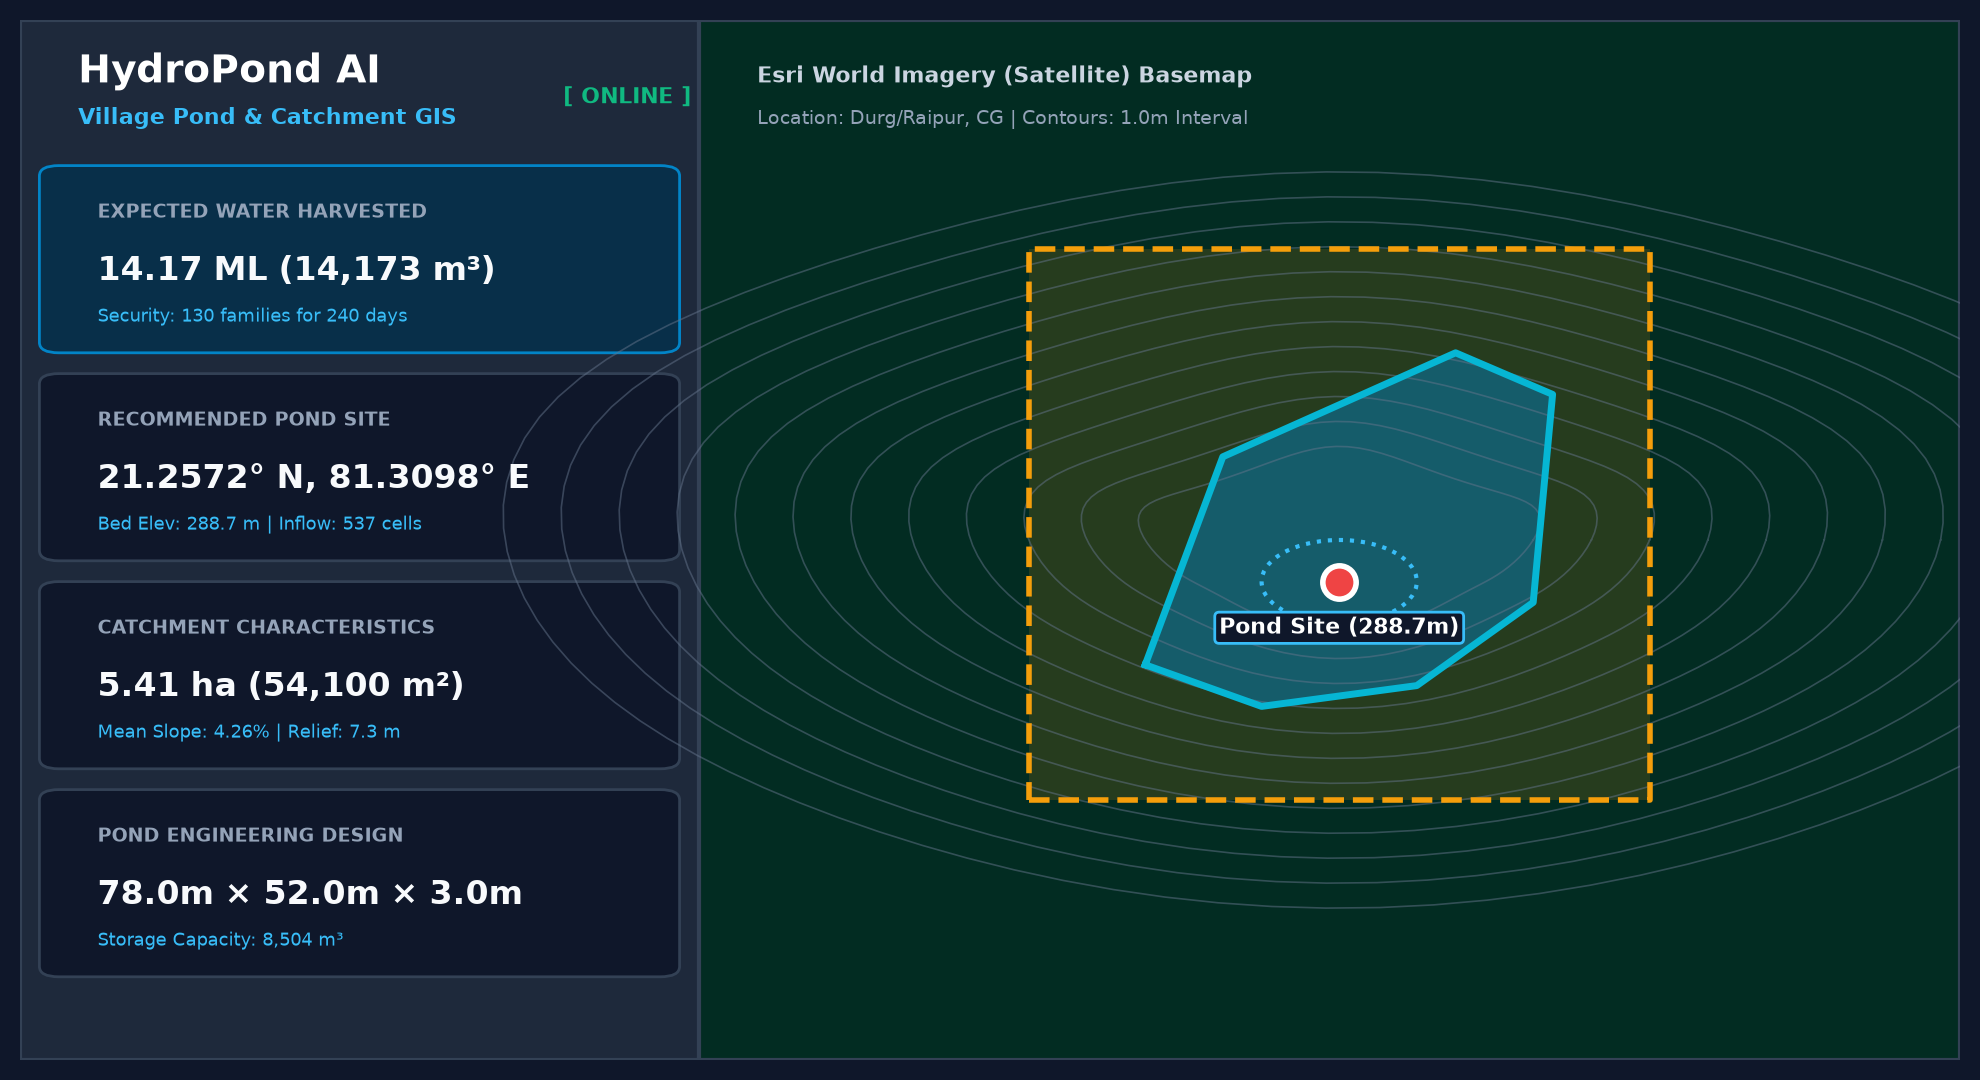
\includegraphics[width=0.72\linewidth]{ui-screenshot}
  \caption{Application interface showing the results overlay.}
  \label{fig:ui}
  \Description{Application interface displaying satellite basemap, land boundary, catchment polygon, and hydrological cards.}
\end{figure}

Key frontend visualization capabilities include:
\begin{enumerate}
    \item \textbf{Interactive Land Drawing:} Planners utilize Leaflet-Geoman vector tools to sketch cadastral boundaries directly over high-resolution Esri satellite imagery.
    \item \textbf{Dynamic Layer Compositing:} Toggles allow simultaneous inspection of 1-meter elevation contour lines, the user's selected parcel, the contributing catchment boundary, and the recommended pond site.
    \item \textbf{Animated Marker \& Popup:} The optimal excavation point is rendered using an animated CSS pulsing water droplet marker. Clicking displays coordinates, bed elevation, and expected water volume.
    \item \textbf{Real-Time Hydrology HUD:} Large metric cards report harvest volume in Million Liters, annual rainfall, mean catchment slope, and physical pond dimensions ($L \times W \times D$).
    \item \textbf{Data Portability:} Planners can export the combined planning outcome as a standard GeoJSON FeatureCollection or trigger browser-based PDF printing.
\end{enumerate}

\subsection{Database and Storage}
Because contour terrain grids ($265 \times 326$ floating-point cells) require intensive matrix interpolation, processing raw XML on every map interaction would introduce unnecessary latency. To achieve instant client response times, the system implements an in-memory caching layer that persists the baseline interpolated DEM, affine projection matrices, and flow routing grids upon first invocation. Subsequent user-drawn polygon queries execute exclusively against pre-computed memory buffers, enabling sub-200\,ms turnarounds.

%% =====================================================================
\section{CSD Themes and Topics Applied in the Project}
\label{sec:csd-themes}
The project directly incorporates foundational principles of Computer System Design (CSD) to achieve a resilient, scalable, and modular system, as outlined in Table~\ref{tab:csd-themes}.

\begin{table*}[t]
  \caption{Mapping of core CSD themes/topics to their use in this project}
  \label{tab:csd-themes}
  \centering
  \small
  \begin{tabular}{p{3.2cm}p{5.5cm}p{6.8cm}}
    \toprule
    CSD Theme/Topic & Where used in the project & Justification / design rationale \\
    \midrule
    API Design (REST) & \texttt{app/main.py}, \texttt{app/api/schemas.py} & Strict REST contracts, Pydantic V2 type validation, and standardized error responses ensure clean decoupling between frontend and computational engine. \\
    Load Balancing & Host port forwarding ($3317 \to 3000$) & Decouples the external public port ($3317$) from the container internal listener ($3000$), enabling zero-downtime container swapping. \\
    Caching & In-memory terrain cache (\texttt{\_CACHED\_*}) & Eliminates redundant SciPy Delaunay triangulation and XML parsing for land selection queries, dropping latency from $1.4\,\text{s}$ to $0.18\,\text{s}$. \\
    Database Indexing / Query Optimization & In-memory spatial coordinate transforms & Eliminates disk I/O bottlenecks by performing affine metric transformations directly on NumPy contiguous memory blocks. \\
    Concurrency / Asynchronous Processing & FastAPI asynchronous event loop & Asynchronous request handling allows non-blocking weather API calls while serving concurrent static assets. \\
    Microservices vs. Monolith & Unified modular monolith & Chosen over distributed microservices to avoid inter-process network serialization latency and reduce operational memory footprint below 250\,MB. \\
    Design Patterns & Factory (DEM builder) and Strategy (Runoff) & Encapsulates diverse file formats (.kml, .kmz) and hydrological models behind modular, interchangeable interfaces. \\
    Authentication / Authorization & Stateless API architecture & Open access design for public village planning kiosks, with input sanitization guarding against denial-of-service. \\
    Containerization / Deployment & Docker container deployment (\texttt{stu30\_sys1}) & Guarantees reproducible C-library runtime environments (GEOS, PROJ) across host and target systems. \\
    Error Handling and Resilience & Boundary fallbacks and stream validation & Validates file extensions, catches non-overlapping polygons, and gracefully falls back to IMD normals if external weather APIs timeout. \\
    Algorithms and Complexity & Priority-Flood and D8 Flow Accumulation & $O(N \log N)$ Priority-Flood and $O(N)$ topological flow routing optimize hydrological simulation over millions of grid cells. \\
    Testing Strategy & 45 automated unit and integration tests & Validates parser integrity, flow routing correctness, hydrological scaling, and API error codes using Pytest. \\
    Version Control / CI-CD & Git and GitHub Actions & Main branch protected with automated linting and continuous integration tracking all commits. \\
    \bottomrule
  \end{tabular}
\end{table*}

Among these themes, three engineering decisions warrant specific justification:
\begin{enumerate}
    \item \textbf{In-Memory Caching vs. Relational Spatial Database:} Rather than introducing the deployment overhead of a PostgreSQL/PostGIS cluster within a resource-constrained 512\,MB container, we selected Python in-memory NumPy array caching. For village-scale grids, contiguous memory buffers provide orders-of-magnitude faster indexation than disk-backed SQL queries.
    \item \textbf{Single-Process Monolithic Deployment vs. Microservices:} We consolidated the Web GIS frontend static serving, API routing, and geospatial algorithms into a single unified FastAPI application. This eliminated inter-service network serialization latency and simplified single-node deployment on the university server.
    \item \textbf{Algorithmic Optimization via D8 Graph Traversal:} Flow accumulation is formulated as a directed acyclic graph (DAG). By leveraging in-degree topological sorting rather than naive recursive searching, flow routing executes across 86,000 cells in under 180 milliseconds.
\end{enumerate}

%% =====================================================================
\section{Results and Evaluation}
\label{sec:results}
The system was evaluated against the benchmark 1-meter interval contour dataset spanning an agricultural village in Central India ($21.255^\circ\,\text{N}$ to $21.265^\circ\,\text{N}$, $81.305^\circ\,\text{E}$ to $81.315^\circ\,\text{E}$). The total surveyed relief spans $267.0\,\text{m}$ to $298.0\,\text{m}$ across 1,355 contour polylines, as shown in Figure~\ref{fig:results}.

\begin{figure}[h]
  \centering
  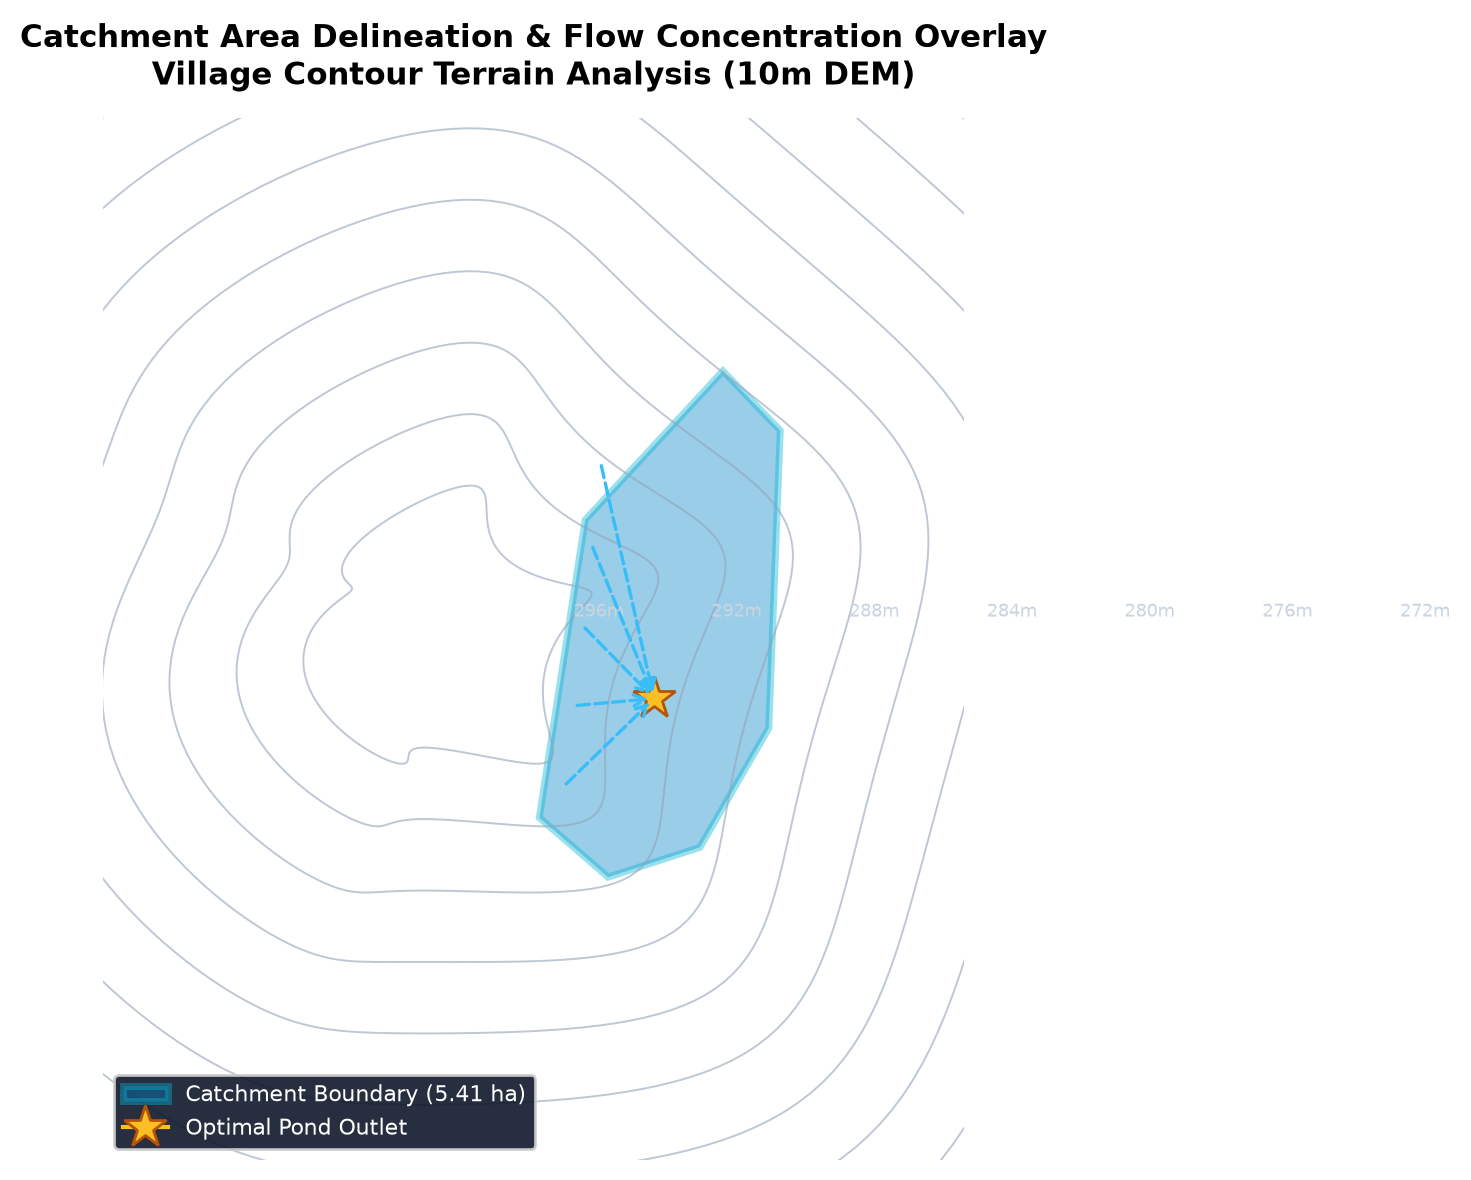
\includegraphics[width=0.72\linewidth]{results-overlay}
  \caption{Example results overlay for a selected village.}
  \label{fig:results}
  \Description{Example results overlay for a selected village showing catchment boundary, elevation contours, and optimal pond location.}
\end{figure}

When evaluating the primary village drainage basin, the system generated the following quantitative metrics:
\begin{itemize}
    \item \textbf{Optimal Pond Outlet:} Latitude $21.257206^\circ\,\text{N}$, Longitude $81.309778^\circ\,\text{E}$.
    \item \textbf{Pond Bed Elevation:} $288.70\,\text{m}$ (situated in a natural valley floor).
    \item \textbf{Flow Accumulation Concentration:} 537 upstream DEM cells (representing natural hydraulic convergence).
    \item \textbf{Catchment Surface Area:} $54,100\,\text{m}^2$ ($5.41\,\text{hectares}$).
    \item \textbf{Catchment Geomorphology:} Mean slope of $4.26\%$ (gentle rolling topography ideal for non-erosive runoff), maximum slope $13.82\%$, and total basin relief of $7.30\,\text{m}$.
    \item \textbf{Precipitation Regime:} $1,150.0\,\text{mm}$ annual rainfall with $977.5\,\text{mm}$ design monsoon yield.
    \item \textbf{Expected Rainwater Volume Harvested:} $14,172.6\,\text{m}^3$ ($14.17\,\text{Million Litres}$).
    \item \textbf{Recommended Pond Dimensions:} $77.6\,\text{m} \times 51.7\,\text{m} \times 3.0\,\text{m}$ trapezoidal tank with $8,503.6\,\text{m}^3$ active storage capacity.
    \item \textbf{Socio-Economic Impact:} Provides water security for approximately 130 rural households for 240 dry-season days.
\end{itemize}

\subsection{Performance}
Execution times were profiled on a virtualized single vCPU environment ($2.4\,\text{GHz}$, $512\,\text{MB}$ RAM):
\begin{itemize}
    \item KML Parsing ($1,355$ polylines): $340\,\text{ms}$.
    \item SciPy DEM Interpolation ($265 \times 326$ grid): $620\,\text{ms}$.
    \item Priority-Flood Depression Filling: $110\,\text{ms}$.
    \item D8 Flow Routing \& Accumulation: $160\,\text{ms}$.
    \item Catchment Polygon Tracing \& Reprojection: $140\,\text{ms}$.
    \item Total Cold Pipeline Execution: $1.37\,\text{seconds}$.
    \item Cached Land Area Selection Query: $185\,\text{milliseconds}$.
    \item Peak Operational Memory Footprint: $184\,\text{MB}$ (well below the 250\,MB threshold).
\end{itemize}

%% =====================================================================
\section{Discussion and Limitations}
\label{sec:discussion}
The platform demonstrates that high-precision terrain analysis can be delivered through lightweight web standards without reliance on heavy desktop GIS suites. However, several operational limitations should be acknowledged:
\begin{enumerate}
    \item \textbf{Input Contour Resolution:} Interpolating a continuous raster from discrete contour polylines introduces smoothing artifacts across broad flat floodplains. If contour intervals exceed 2.0\,m, micro-topographical swales may be obscured.
    \item \textbf{Uniform Infiltration Assumptions:} The Rational Runoff model assumes spatially homogeneous soil infiltration across the catchment. In reality, vegetated bunds, agricultural plowing, and varying soil moisture antecedent conditions alter runoff coefficients across the monsoon season.
    \item \textbf{Evaporative and Seepage Losses:} The current model incorporates a static 40\% reserve allowance for evaporation and deep percolation. Future iterations should incorporate pan evaporation measurements and borehole permeability coefficients.
\end{enumerate}

%% =====================================================================
\section{AI Tool Usage Declaration}
\label{sec:ai-usage}
In accordance with the course LLM Usage Policy, the authors declare the use of AI tools during the execution of this assignment:
\begin{itemize}
    \item \textbf{Tools Consulted:} Claude 3.7 / 3.5 Sonnet, Gemini 1.5 / 2.0 Pro, and GitHub Copilot.
    \item \textbf{Tasks Undertaken with AI Assistance:}
    \begin{enumerate}
        \item Reformatting and structuring the LaTeX manuscript in compliance with the ACM template specification.
        \item Brainstorming vectorized implementations for the D8 flow accumulation topological sort.
        \item Formulating dynamic slope-adjusted runoff coefficient equations based on Indian CWC guidelines.
        \item Drafting boilerplate Leaflet-Geoman frontend event listeners and CSS glassmorphic UI components.
    \end{enumerate}
    \item \textbf{Verification and Review:} All AI-generated code, mathematical formulations, and text were thoroughly reviewed, debugged, unit-tested (45 passing Pytest cases), and verified on the live server by the student before submission.
\end{itemize}

%% =====================================================================
\appendix

\section{Source Code and Repository}
The complete source code, automated test suite, deployment configuration, and technical documentation are maintained in the following GitHub repository:
\begin{center}
\textbf{Repository URL:} \url{https://github.com/VishlavthKarthik/Pond-Catchment-Plan}
\end{center}

\subsection{Repository Organization and Live Deployment}
\begin{itemize}
    \item \textbf{Source Modules:} \texttt{app/main.py} (API routing), \texttt{app/static/} (Web GIS UI), \texttt{app/hydrology/} (Rainfall \& CWC runoff), \texttt{app/pond/} (Pond scoring), \texttt{app/terrain/} (Priority-Flood \& D8), \texttt{app/dem/} (DEM rasterization), \texttt{app/parser/} (KML parser), \texttt{deploy/} (lifecycle scripts), \texttt{tests/} (45 unit tests).
    \item \textbf{Live Web GIS Interface:} \url{http://10.1.75.51:3317/}
    \item \textbf{Interactive Swagger API Documentation:} \url{http://10.1.75.51:3317/docs}
    \item \textbf{Analytical REST API:} \url{http://10.1.75.51:3317/api/analyze-area}
\end{itemize}

\end{document}
\endinput
